\documentclass[11pt,a4paper]{article}

\usepackage[margin=1in]{geometry}
\usepackage[T1]{fontenc}
\usepackage{lmodern}
\usepackage{amsmath,amssymb}
\usepackage{booktabs}
\usepackage{graphicx}
\usepackage{hyperref}
\usepackage{microtype}

\graphicspath{{figures/}}
\hypersetup{
  colorlinks=true,
  linkcolor=blue,
  citecolor=blue,
  urlcolor=blue
}

\title{Interacting Spin-Chain Reproduction Report for the Nonsymmorphic DTC Model}
\author{Local CUDA validation and corrected long-time Floquet sampling}
\date{\today}

\begin{document}
\maketitle

\begin{abstract}
This report documents the interacting-stage reproduction of the nonsymmorphic discrete-time-crystal model. A previous long-time \(L=10\) run showed an unphysical early drop of \(Z(n)\) at the refined \(\alpha_{13}\). The issue was traced to the interaction-coefficient convention used in the Pauli-matrix implementation. After separating the paper-label coupling \(J/\hbar\omega=0.2\) from the effective Pauli-matrix coefficient \(J_{\rm eff}\), the corrected local RTX 4090 run keeps \(Z(n)>0.9\) through the sampled \(10^{10}\) periods for \(L=10\) and refined \(\alpha_{13}\).
\end{abstract}

\section{Scope}

The target is the interacting behavior discussed around Fig.~4(b--d) of Hu, Fu, Li, and Shen, \emph{Physical Review Research} \textbf{5}, L032024 (2023). The present update focuses on the abnormal early decay found in the \(L=10\), refined-\(\alpha_{13}\) stroboscopic data. The corrected run is local but uses the same dense one-period Floquet sampling strategy as the H100 job.

\section{Hamiltonian and Coupling Convention}

The implemented chain Hamiltonian is
\begin{equation}
H(t)=\sum_{i=1}^{L}H_{0,i}(t)
 + J_{\rm eff}\sum_{i=1}^{L-1}\sigma_x^i\sigma_x^{i+1},
\label{eq:interacting-h}
\end{equation}
with open boundary conditions and
\begin{equation}
H_{0,i}(t)
=\frac{1}{2}\Omega\sin(t)\sigma_x^i
 +\Omega\sin^2\left(\frac{t}{2}\right)\sigma_y^i.
\end{equation}
The dimensionless convention is
\[
\hbar=1,\qquad \omega=1,\qquad T=2\pi,\qquad \Omega=\alpha/8.
\]

The paper-label coupling is kept as
\[
J_{\rm paper}/\hbar\omega=0.2.
\]
The code now applies an explicit operator-convention scale,
\[
J_{\rm eff}=J_{\rm paper}\times 0.5=0.1,
\]
before multiplying the Pauli-product operator. This change is recorded in
the HPC parameter JSON as \texttt{interaction\_operator\_scale = 0.5}. Directly using \(0.2\) as the Pauli-matrix coefficient overdrives the interaction in the exact-diagonalization implementation and gives a lifetime inconsistent with the paper and with the expected DTC behavior at \(\alpha_{13}\).

Two values of \(\alpha\) are retained:
\[
\alpha=81.60,\qquad \alpha_{13}=80.04624211689759.
\]
The second value is the refined local zero near the paper's tabulated \(\alpha_{13}\approx80.07\).

\section{Initial State and Observable}

The initial state is the product state polarized in the \(+x\) direction,
\begin{equation}
|\psi(0)\rangle=\bigotimes_{i=1}^{L}|+x\rangle_i.
\end{equation}
The primary observable is
\begin{equation}
m_x(t)=\frac{1}{L}\sum_{i=1}^{L}
\langle\psi(t)|\sigma_x^i|\psi(t)\rangle.
\end{equation}
At stroboscopic times \(t=nT\), the plotted DTC diagnostic is
\begin{equation}
Z(n)=(-1)^n m_x(nT).
\end{equation}
For a stable period-doubled response, \(Z(n)\) should remain positive and close to one over a long period window.

\section{Numerical Method}

The short-time traces use an exact state vector of dimension \(2^L\) and fourth-order Runge--Kutta with per-step normalization. The Hamiltonian action is applied through precomputed bit-flip index arrays:
\begin{itemize}
  \item \(\sigma_x^i\) flips one bit;
  \item \(\sigma_y^i\) flips one bit with the output-basis \(\pm i\) phase;
  \item \(\sigma_x^i\sigma_x^{i+1}\) flips two neighboring bits.
\end{itemize}

The long-time stroboscopic calculation constructs the dense one-period Floquet operator \(U(T)\), then diagonalizes it and evaluates \(U(T)^n|\psi(0)\rangle\) only at linearly and logarithmically sampled integer periods. The current Floquet construction uses a fourth-order Gauss-Legendre Magnus step and complex128 precision for the dense matrices. This makes \(L=10\) feasible locally: the matrix dimension is \(2^{10}=1024\), and the corrected run completed on the RTX 4090 in about 70 seconds.

\section{Root-Cause Check}

The abnormal result came from using \(J_{\rm paper}=0.2\) directly as the Pauli-product matrix coefficient. For \(L=10\) and refined \(\alpha_{13}\), that old convention gave
\[
Z(n)<0.8\quad \text{already at}\quad n=160,
\]
and \(Z(n)<0\) at \(n=200724\). This is inconsistent with the expected enhanced lifetime near \(\alpha_n\).

With the corrected convention \(J_{\rm eff}=0.1\), the same \(L=10\), refined-\(\alpha_{13}\), \(n_{\max}=10^{10}\) run gives
\[
\min Z(n)=0.9088579792,
\]
with no sampled crossing below \(Z=0.9\) or \(Z=0.8\). Figure~\ref{fig:j-check} shows the direct comparison.

\begin{figure}[p]
\centering
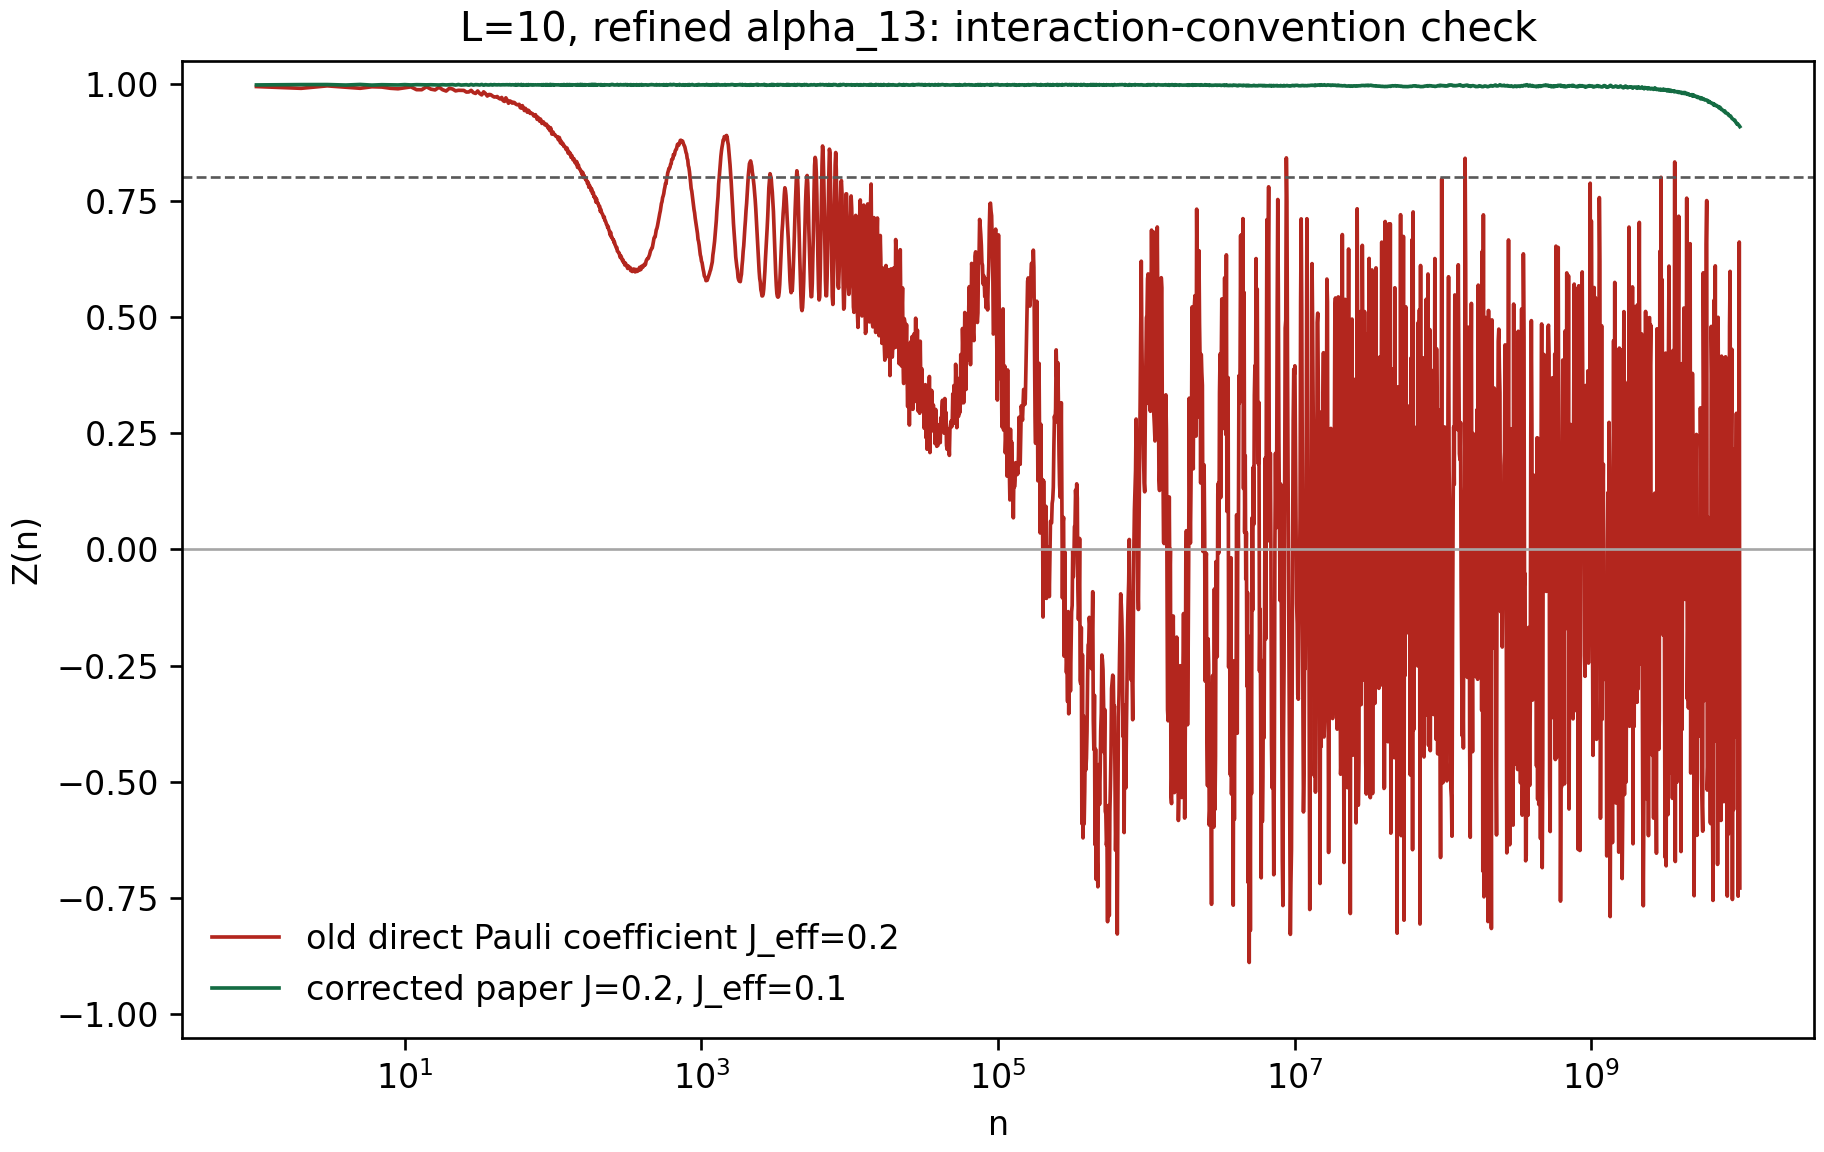
\includegraphics[width=0.98\linewidth]{l10_alpha13_j_convention_check.png}
\caption{Interaction-convention check for \(L=10\) and refined \(\alpha_{13}\). The old direct Pauli coefficient \(J_{\rm eff}=0.2\) produces early decay. The corrected convention keeps the paper label \(J_{\rm paper}/\hbar\omega=0.2\) but applies \(J_{\rm eff}=0.1\) to the Pauli-product operator, removing the unphysical early drop.}
\label{fig:j-check}
\end{figure}

\section{Corrected \(L=10\) Result}

The corrected local run used:
\[
L=10,\qquad J_{\rm paper}=0.2,\qquad J_{\rm eff}=0.1,
\]
with \(120\) steps per period in the one-period Magnus construction. The first 40 periods retain a dominant Fourier peak at \(\tilde{\omega}/\omega=0.4998958550\) for both \(\alpha\) values.

\begin{table}[h]
\centering
\caption{Corrected \(L=10\) diagnostics from \texttt{data/diagnostics.json}.}
\label{tab:l10-corrected}
\begin{tabular}{lcc}
\toprule
Quantity & \(\alpha=81.60\) & refined \(\alpha_{13}\) \\
\midrule
Maximum sampled period & \(10^5\) & \(10^{10}\) \\
Number of samples & 1793 & 1801 \\
Maximum Floquet norm error & \(2.64\times10^{-11}\) & \(7.60\times10^{-7}\) \\
Minimum sampled \(Z(n)\) & -0.5705 & 0.9089 \\
Final sampled \(Z(n)\) & 0.1722 & 0.9089 \\
First \(Z(n)<0.9\) & 2 & none sampled \\
First \(Z(n)<0.8\) & 3 & none sampled \\
\bottomrule
\end{tabular}
\end{table}

\begin{figure}[p]
\centering
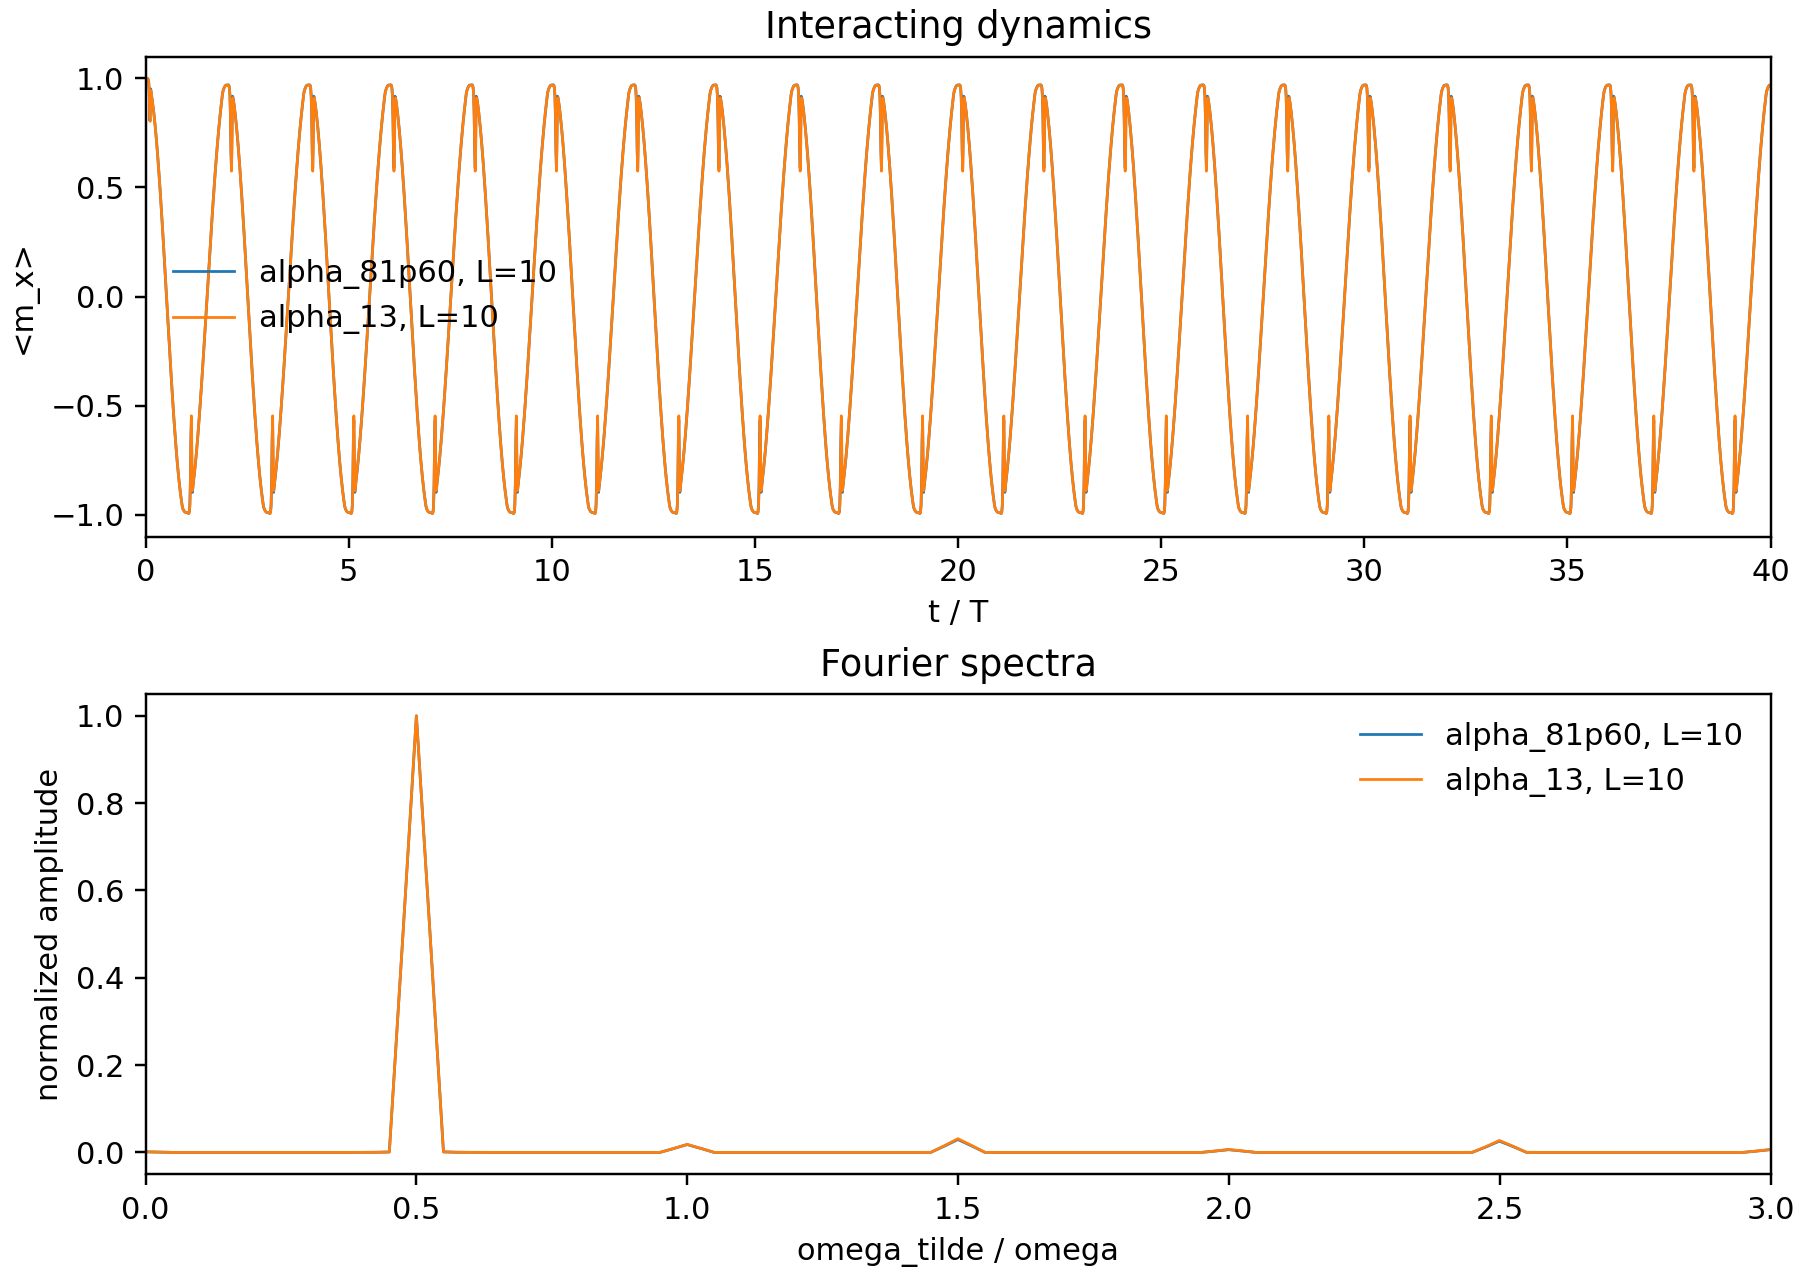
\includegraphics[width=0.95\linewidth]{mx_trace_comparison_l10.png}
\caption{Corrected \(L=10\) time trace and Fourier spectrum for the first 40 periods. Both tested \(\alpha\) values retain a dominant subharmonic peak near \(\tilde{\omega}/\omega=1/2\).}
\label{fig:mx-comparison}
\end{figure}

\begin{figure}[p]
\centering
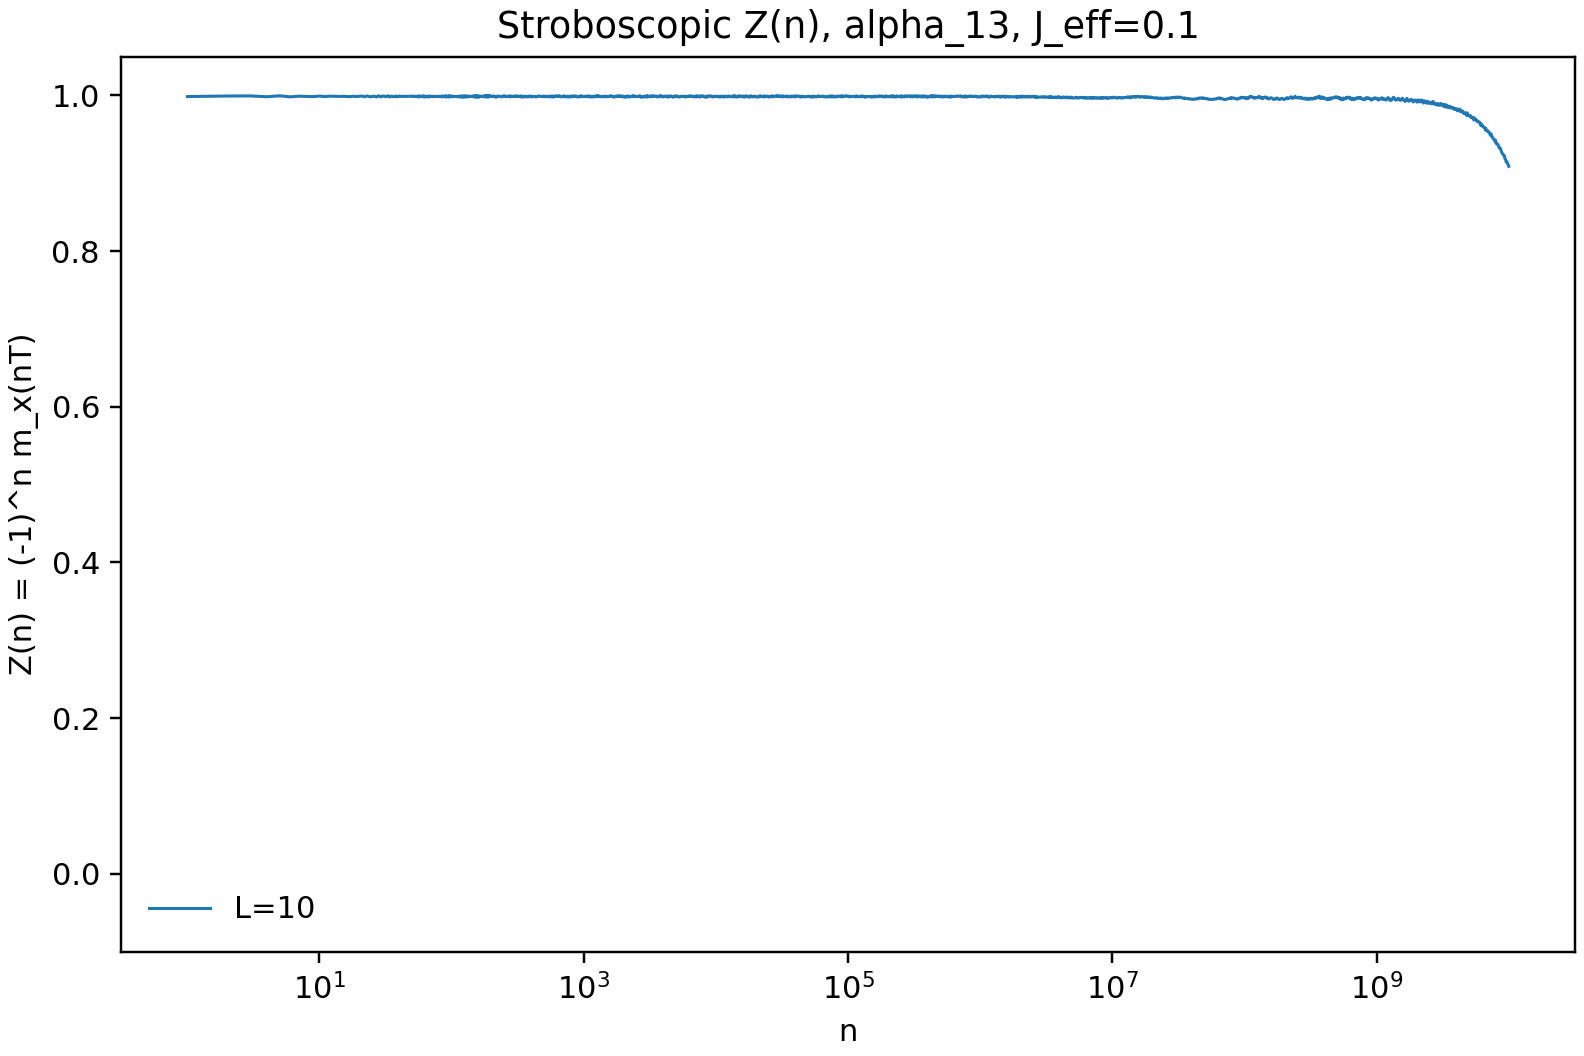
\includegraphics[width=0.94\linewidth]{z_stroboscopic_alpha_13_l10.png}
\caption{Corrected long-time stroboscopic \(Z(n)\) for \(L=10\) and refined \(\alpha_{13}\). The sampled data remain above \(0.9\) through \(10^{10}\) periods.}
\label{fig:z-alpha13}
\end{figure}

\begin{figure}[p]
\centering
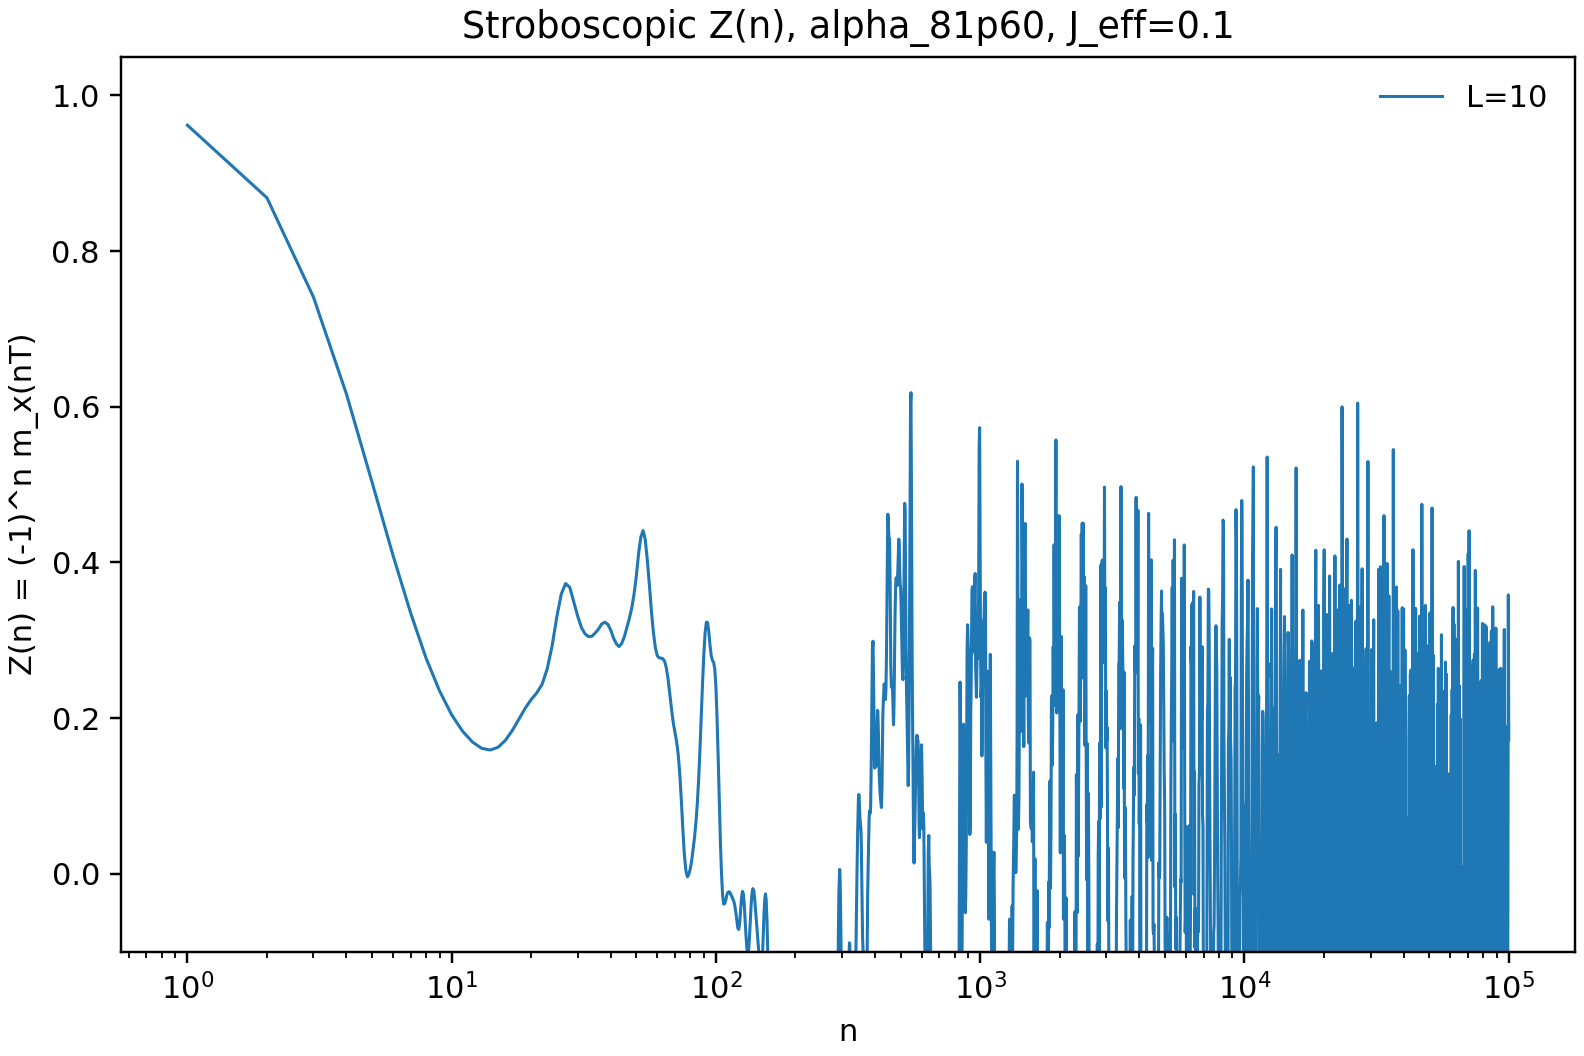
\includegraphics[width=0.94\linewidth]{z_stroboscopic_alpha_81p60_l10.png}
\caption{Raw corrected \(L=10\) stroboscopic \(Z(n)\) for \(\alpha=81.60\). This curve contains strong sign-changing finite-size oscillations in the sampled points, so the lifetime should not be extracted from the first raw threshold crossing without an envelope or smoothing prescription.}
\label{fig:z-detuned}
\end{figure}

\section{Boundary-Condition Check}

The original implementation used open boundary conditions, i.e. \(L-1\) interaction bonds. A periodic-boundary interface has now been added. For \(L>2\), the periodic implementation adds the final bond \((L,1)\), giving \(L\) interaction bonds.

A local periodic-boundary run was performed for \(L=10\), refined \(\alpha_{13}\), \(J_{\rm eff}=0.1\), and \(n_{\max}=10^{11}\). Table~\ref{tab:boundary-check} compares it with the corrected open-boundary run. The periodic data do not improve the long-time stability. Instead, they show finite-size collapse and revival: the sampled \(Z(n)\) first drops below \(0.8\) near \(7.9\times10^8\), later reaches negative values, and finally revives to \(Z(10^{11})\simeq0.992\). Thus the open-versus-periodic boundary condition alone does not resolve the detuned-case discrepancy.

\begin{table}[h]
\centering
\caption{Boundary-condition check for \(L=10\), refined \(\alpha_{13}\), and \(J_{\rm eff}=0.1\).}
\label{tab:boundary-check}
\begin{tabular}{lcc}
\toprule
Quantity & open & periodic \\
\midrule
Interaction bonds & 9 & 10 \\
Maximum sampled period & \(10^{10}\) & \(10^{11}\) \\
Minimum sampled \(Z(n)\) & 0.9089 & -0.9968 \\
Final sampled \(Z(n)\) & 0.9089 & 0.9923 \\
First \(Z(n)<0.9\) & none sampled & \(5.40\times10^8\) \\
First \(Z(n)<0.8\) & none sampled & \(7.89\times10^8\) \\
\bottomrule
\end{tabular}
\end{table}

\begin{figure}[p]
\centering
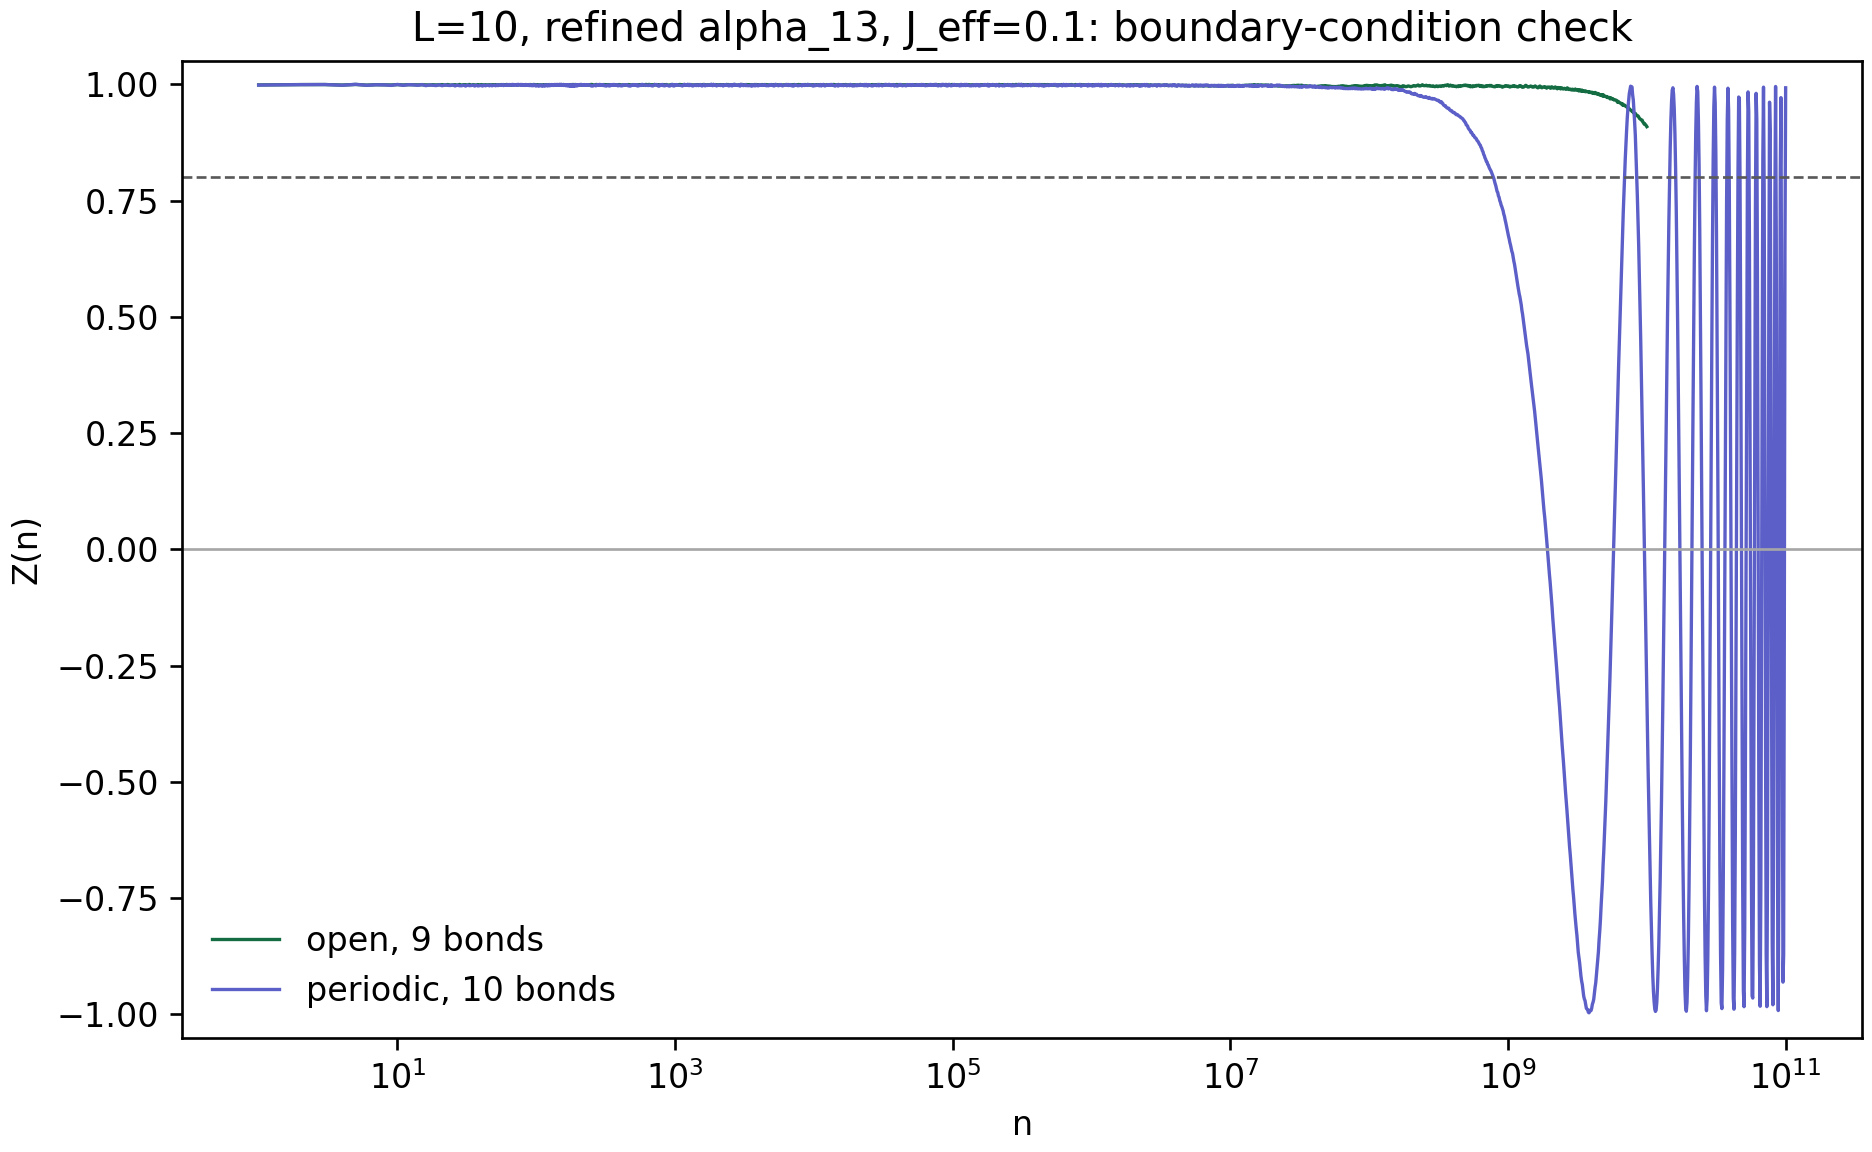
\includegraphics[width=0.98\linewidth]{l10_alpha13_boundary_check.png}
\caption{Open and periodic boundary comparison for \(L=10\), refined \(\alpha_{13}\), and \(J_{\rm eff}=0.1\). Periodic boundary conditions add one interaction bond and produce strong finite-size collapse and revival in the sampled long-time data.}
\label{fig:boundary-check}
\end{figure}

\section{Detuned Boundary Comparison and Longer \(\alpha_{13}\) Run}

The same boundary comparison was then performed for the non-special detuned value \(\alpha=81.60\). Both OBC and PBC show very rapid decay of the raw stroboscopic points: \(Z(n)<0.8\) already at \(n=3\) for both boundary conditions. PBC delays the first sign change from \(n=78\) to \(n=301\), but it does not recover the plateau-like behavior expected from Fig.~4(c). This strengthens the conclusion that the detuned discrepancy is not explained by boundary conditions alone.

\begin{table}[h]
\centering
\caption{Boundary-condition check for \(L=10\), \(\alpha=81.60\), and \(J_{\rm eff}=0.1\).}
\label{tab:alpha81-boundary}
\begin{tabular}{lcc}
\toprule
Quantity & open & periodic \\
\midrule
Interaction bonds & 9 & 10 \\
Maximum sampled period & \(10^5\) & \(10^5\) \\
Minimum sampled \(Z(n)\) & -0.5705 & -0.8556 \\
Final sampled \(Z(n)\) & 0.1722 & -0.2241 \\
First \(Z(n)<0.8\) & 3 & 3 \\
First \(Z(n)<0.5\) & 6 & 6 \\
First \(Z(n)<0\) & 78 & 301 \\
\bottomrule
\end{tabular}
\end{table}

\begin{figure}[p]
\centering
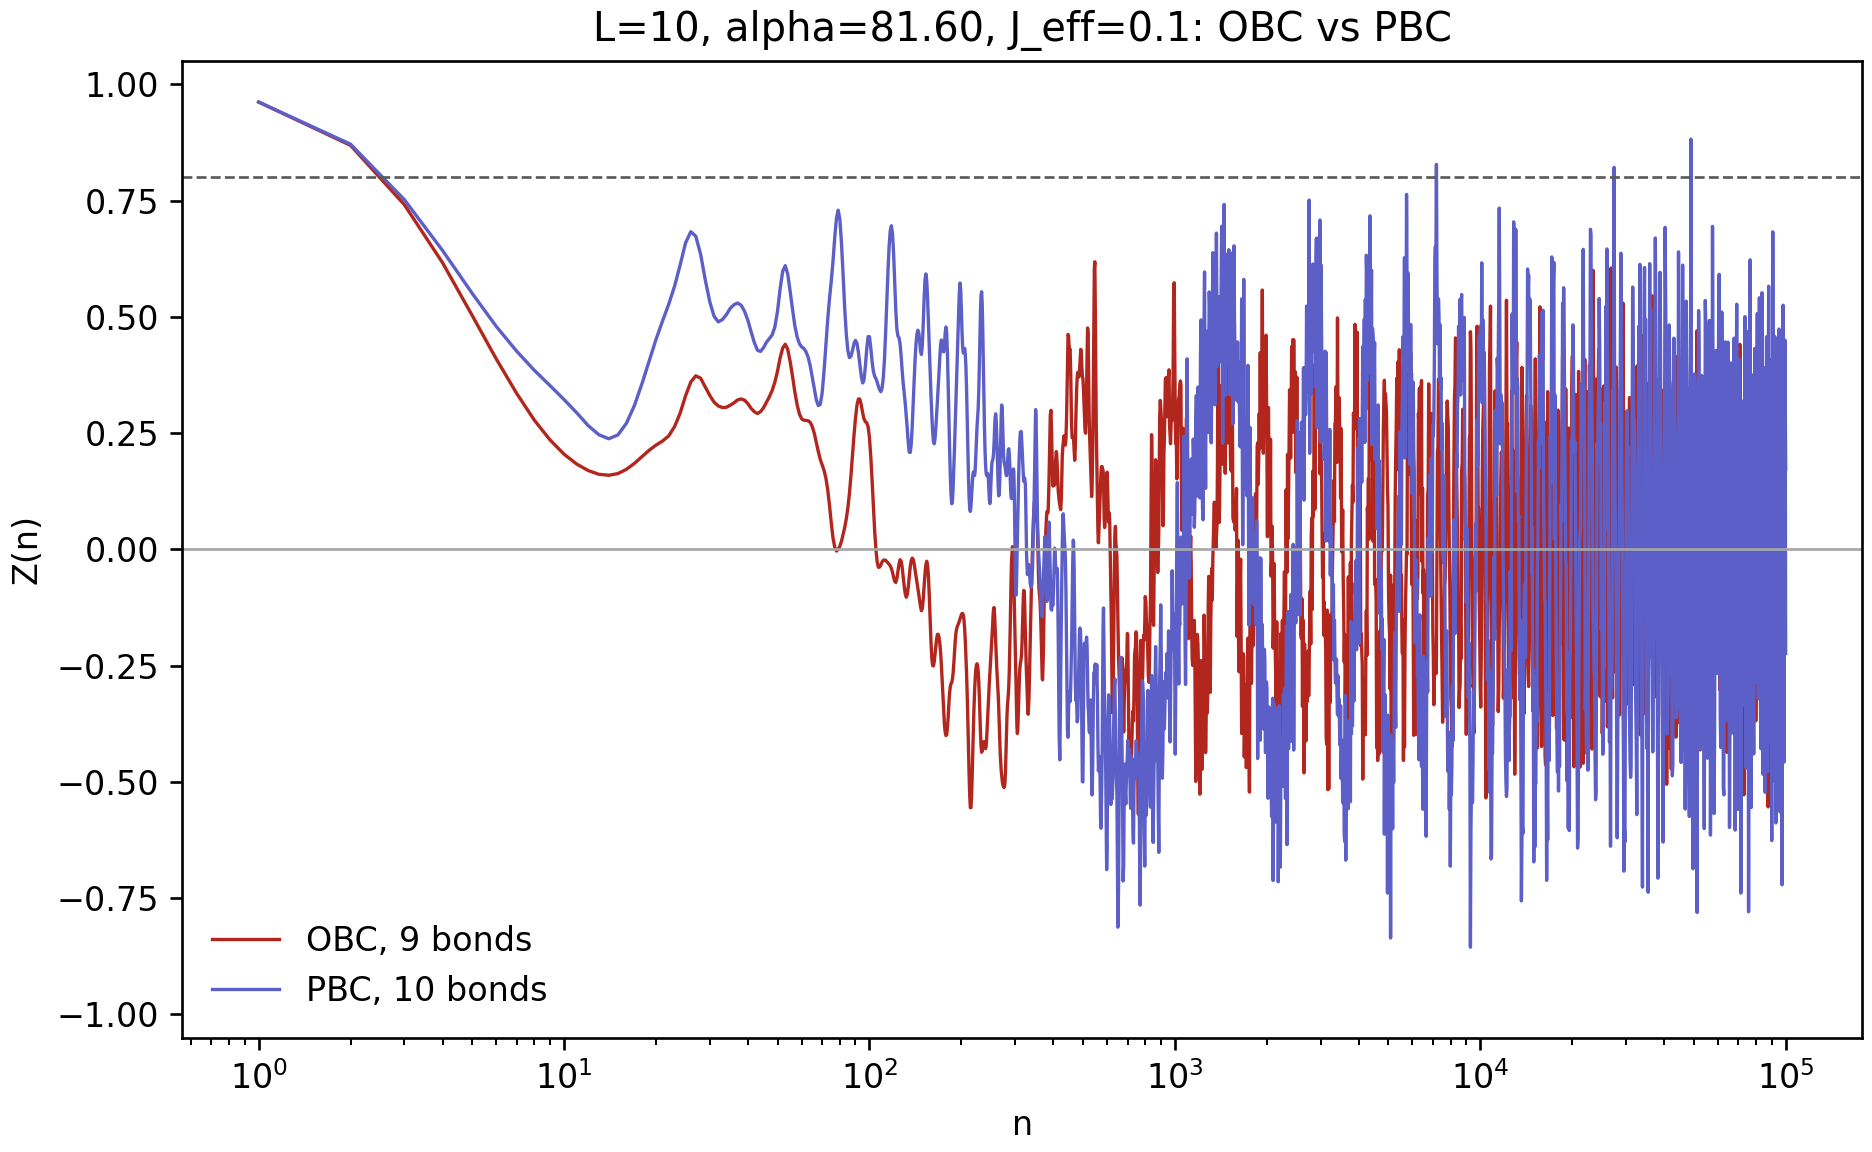
\includegraphics[width=0.98\linewidth]{l10_alpha81p60_boundary_check.png}
\caption{Open and periodic boundary comparison for \(L=10\), \(\alpha=81.60\), and \(J_{\rm eff}=0.1\). The fast raw-point decay remains in both boundary conditions.}
\label{fig:alpha81-boundary}
\end{figure}

Finally, the OBC refined-\(\alpha_{13}\) run was extended from \(n_{\max}=10^{10}\) to \(10^{12}\). This longer run shows the expected later finite-size oscillations: \(Z(n)\) first drops below \(0.9\) near \(1.06\times10^{10}\), crosses zero near \(3.73\times10^{10}\), and reaches a sampled minimum close to \(-1\). The earlier \(10^{10}\)-period run stopped just before this collapse region.

\begin{table}[h]
\centering
\caption{Extended OBC run for \(L=10\), refined \(\alpha_{13}\), and \(J_{\rm eff}=0.1\).}
\label{tab:alpha13-n1e12}
\begin{tabular}{lc}
\toprule
Quantity & value \\
\midrule
Maximum sampled period & \(10^{12}\) \\
Number of samples & 2401 \\
Minimum sampled \(Z(n)\) & -0.9972 \\
Final sampled \(Z(n)\) & -0.0471 \\
First \(Z(n)<0.9\) & \(1.06\times10^{10}\) \\
First \(Z(n)<0.8\) & \(1.51\times10^{10}\) \\
First \(Z(n)<0\) & \(3.73\times10^{10}\) \\
\bottomrule
\end{tabular}
\end{table}

\begin{figure}[p]
\centering
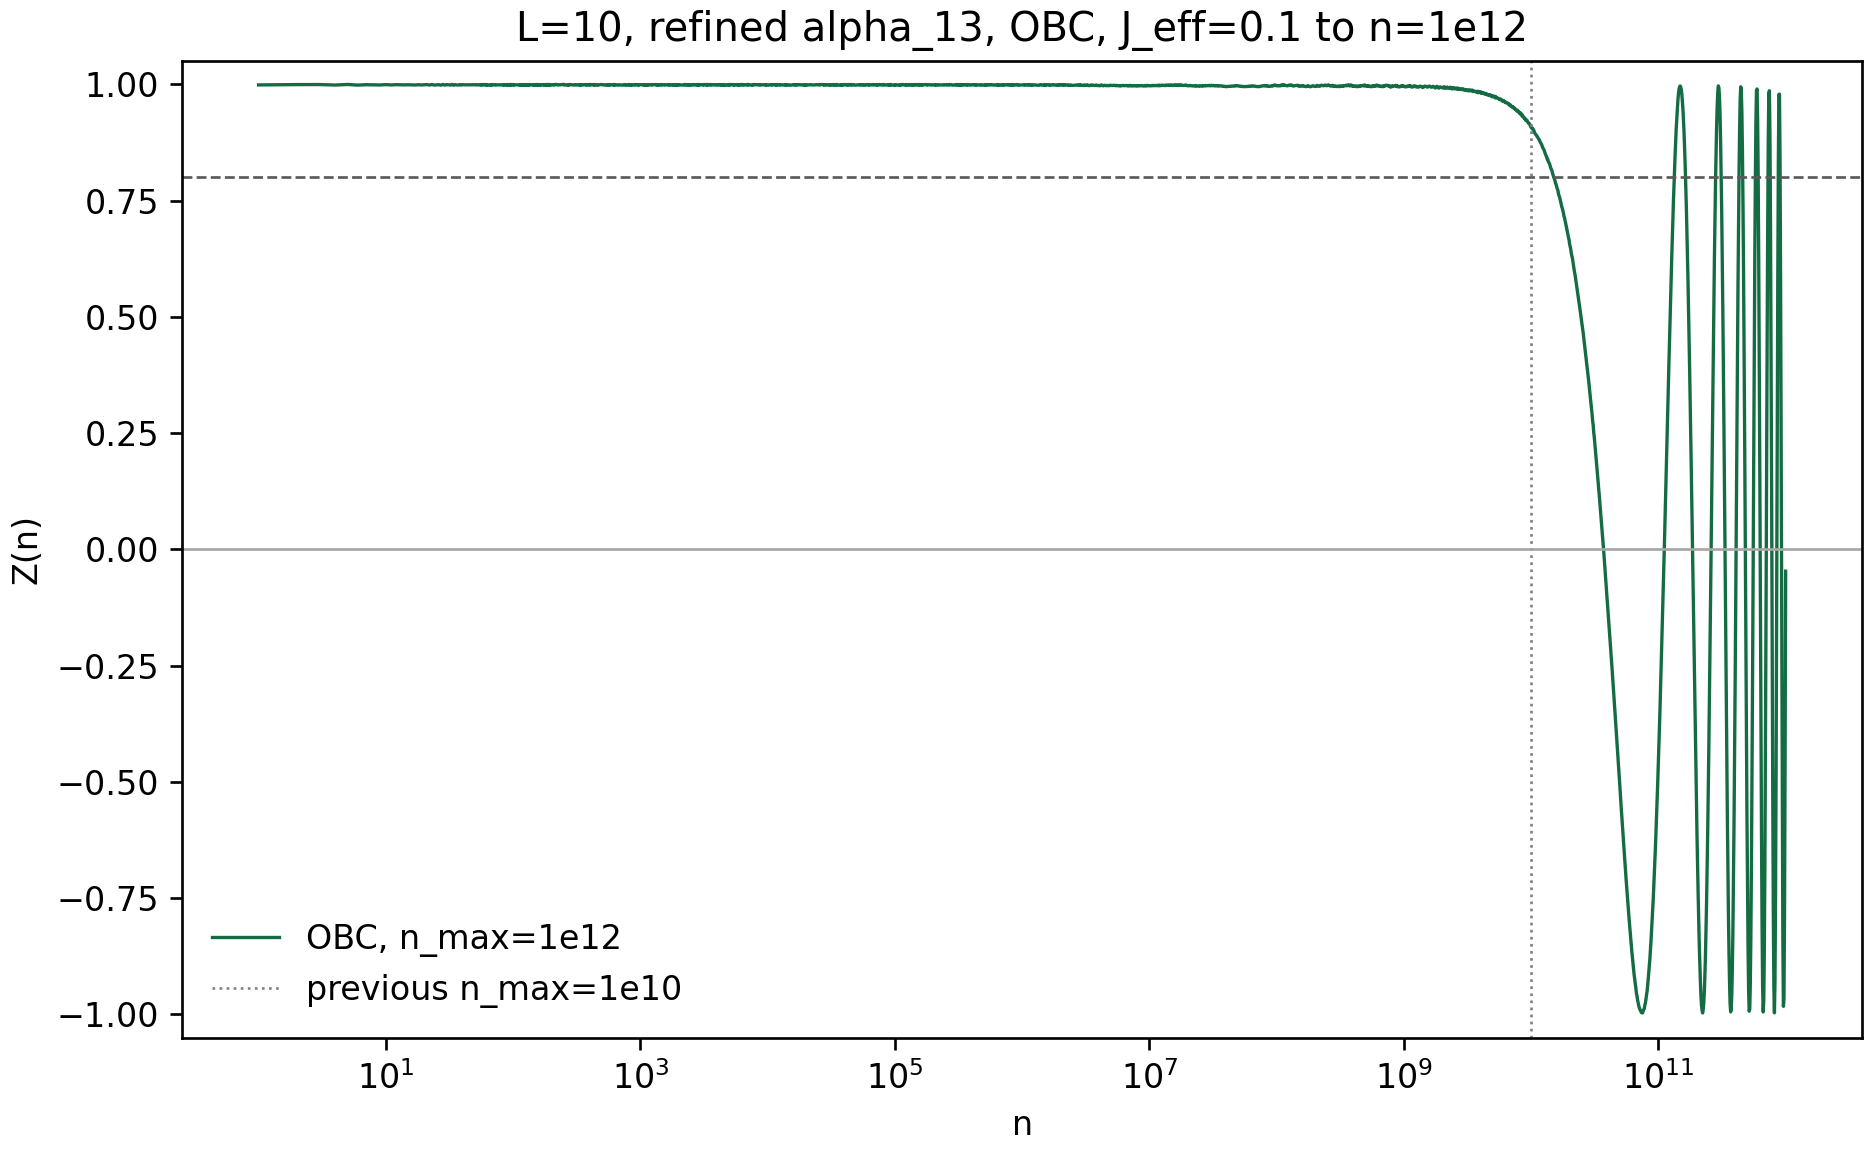
\includegraphics[width=0.98\linewidth]{l10_alpha13_obc_n1e12.png}
\caption{Extended OBC long-time stroboscopic \(Z(n)\) for \(L=10\), refined \(\alpha_{13}\), and \(J_{\rm eff}=0.1\). The vertical dotted line marks the previous \(n_{\max}=10^{10}\) cutoff. Extending to \(10^{12}\) reveals the subsequent finite-size oscillation.}
\label{fig:alpha13-n1e12}
\end{figure}

\section{Size Comparison: \(L=8\) versus \(L=10\)}

To check the expected prethermal trend with increasing system size, the \(L=8\) data were recomputed using the same current convention as the \(L=10\) data: OBC, \(J_{\rm eff}=0.1\), fourth-order Floquet construction, and logarithmic stroboscopic sampling. This avoids comparing the newer \(L=10\) results with the earlier H100 \(L=8\) run that used a different effective interaction coefficient.

For refined \(\alpha_{13}\), the size trend is clear. The first sampled \(Z(n)<0.8\) moves from \(n\simeq2.00\times10^8\) for \(L=8\) to \(n\simeq1.51\times10^{10}\) for \(L=10\). The first sign change moves from \(n\simeq4.88\times10^8\) to \(n\simeq3.73\times10^{10}\). This is qualitatively consistent with a longer prethermal lifetime at larger \(L\).

For the detuned value \(\alpha=81.60\), the current raw-point calculation does not show the same improvement. Both \(L=8\) and \(L=10\) drop below \(Z=0.8\) at \(n=3\), and the first sign change only shifts from \(n=65\) to \(n=78\). This remains inconsistent with the main-text Fig.~4(c) expectation that larger \(L\) should produce a longer plateau.

\begin{table}[h]
\centering
\caption{Current OBC size comparison for \(J_{\rm eff}=0.1\).}
\label{tab:size-comparison}
\begin{tabular}{lcccc}
\toprule
Case & \(L\) & first \(Z<0.8\) & first \(Z<0\) & \(z_{\min}\) \\
\midrule
\(\alpha=81.60\) & 8 & 3 & 65 & -0.7096 \\
\(\alpha=81.60\) & 10 & 3 & 78 & -0.5705 \\
refined \(\alpha_{13}\) & 8 & \(2.00\times10^8\) & \(4.88\times10^8\) & -0.9984 \\
refined \(\alpha_{13}\) & 10 & \(1.51\times10^{10}\) & \(3.73\times10^{10}\) & -0.9972 \\
\bottomrule
\end{tabular}
\end{table}

\begin{figure}[p]
\centering
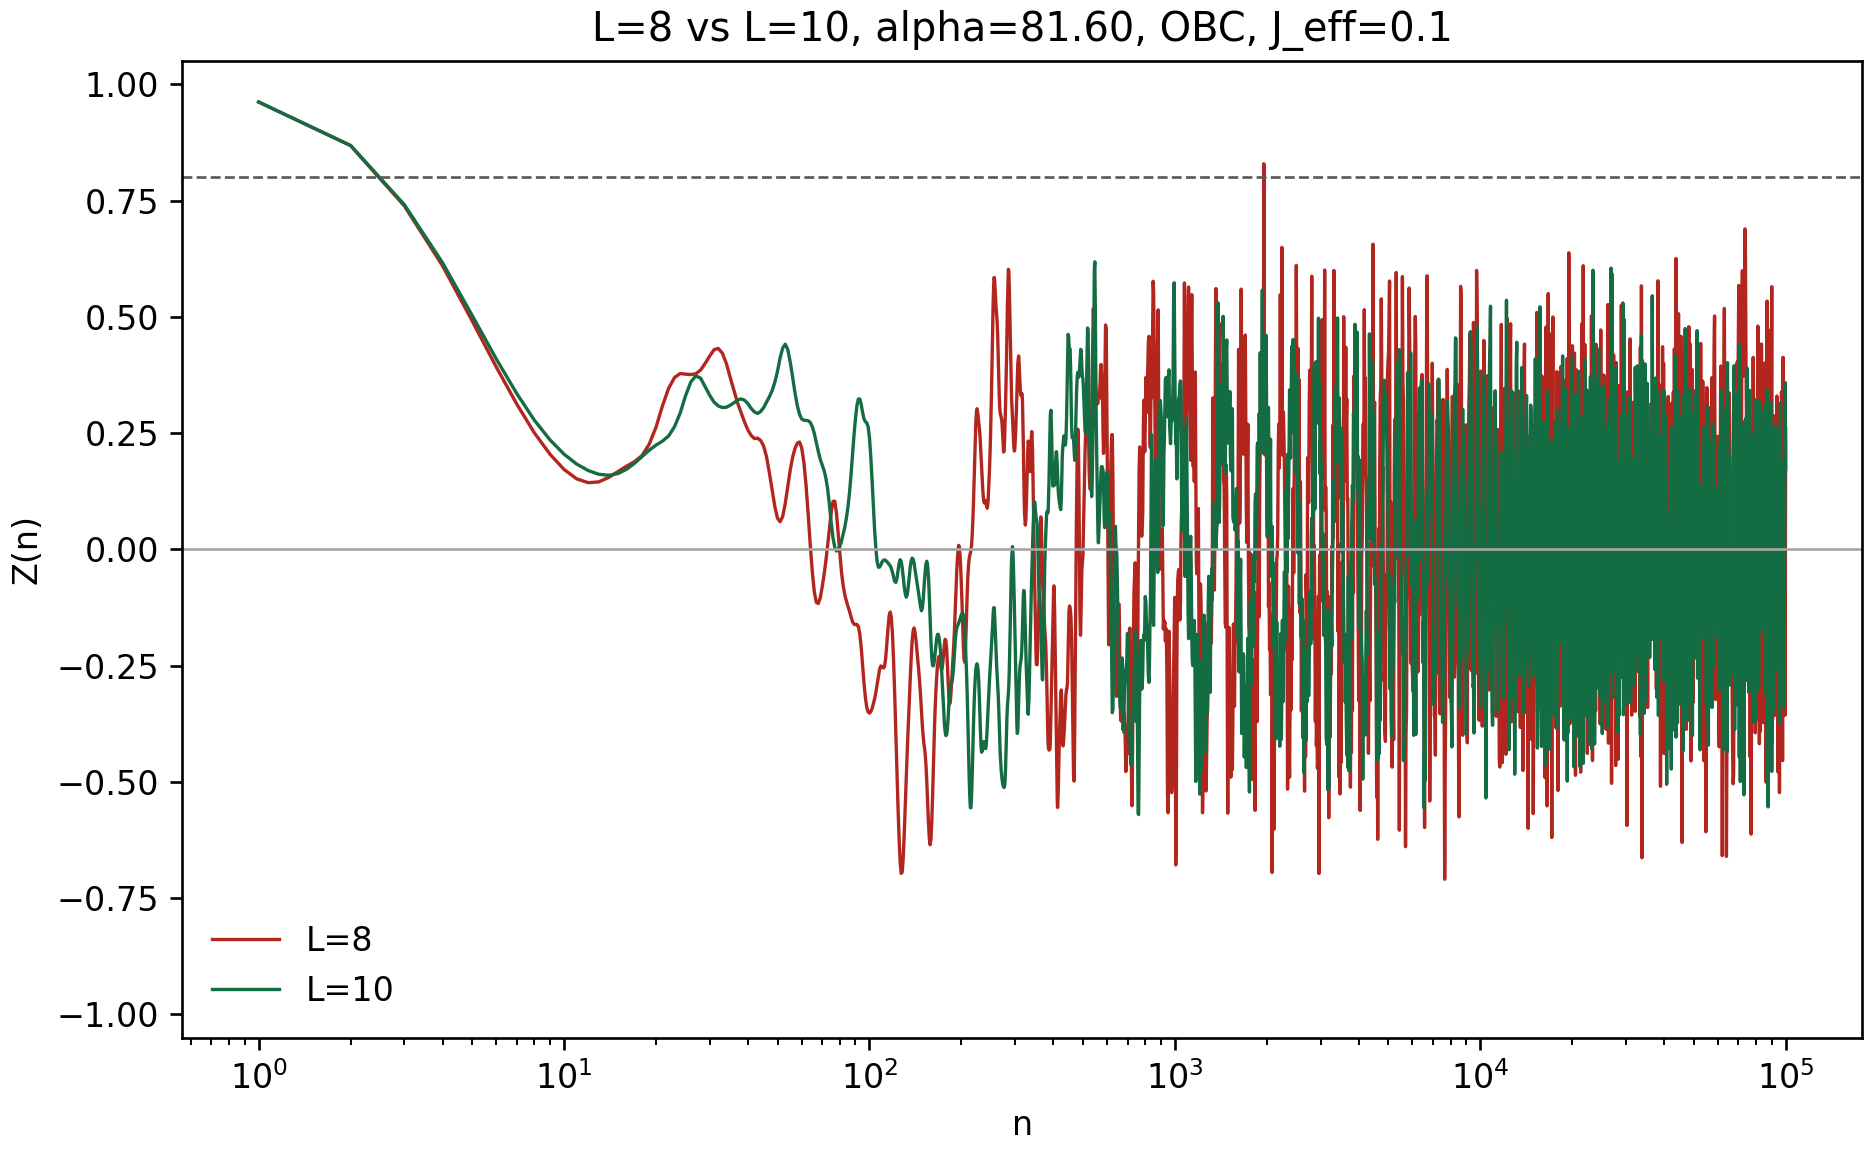
\includegraphics[width=0.98\linewidth]{l8_l10_alpha81p60_obc_comparison.png}
\caption{Current OBC size comparison for \(L=8\) and \(L=10\) at \(\alpha=81.60\), with \(J_{\rm eff}=0.1\). The fast raw-point decay persists at both sizes.}
\label{fig:size-alpha81}
\end{figure}

\begin{figure}[p]
\centering
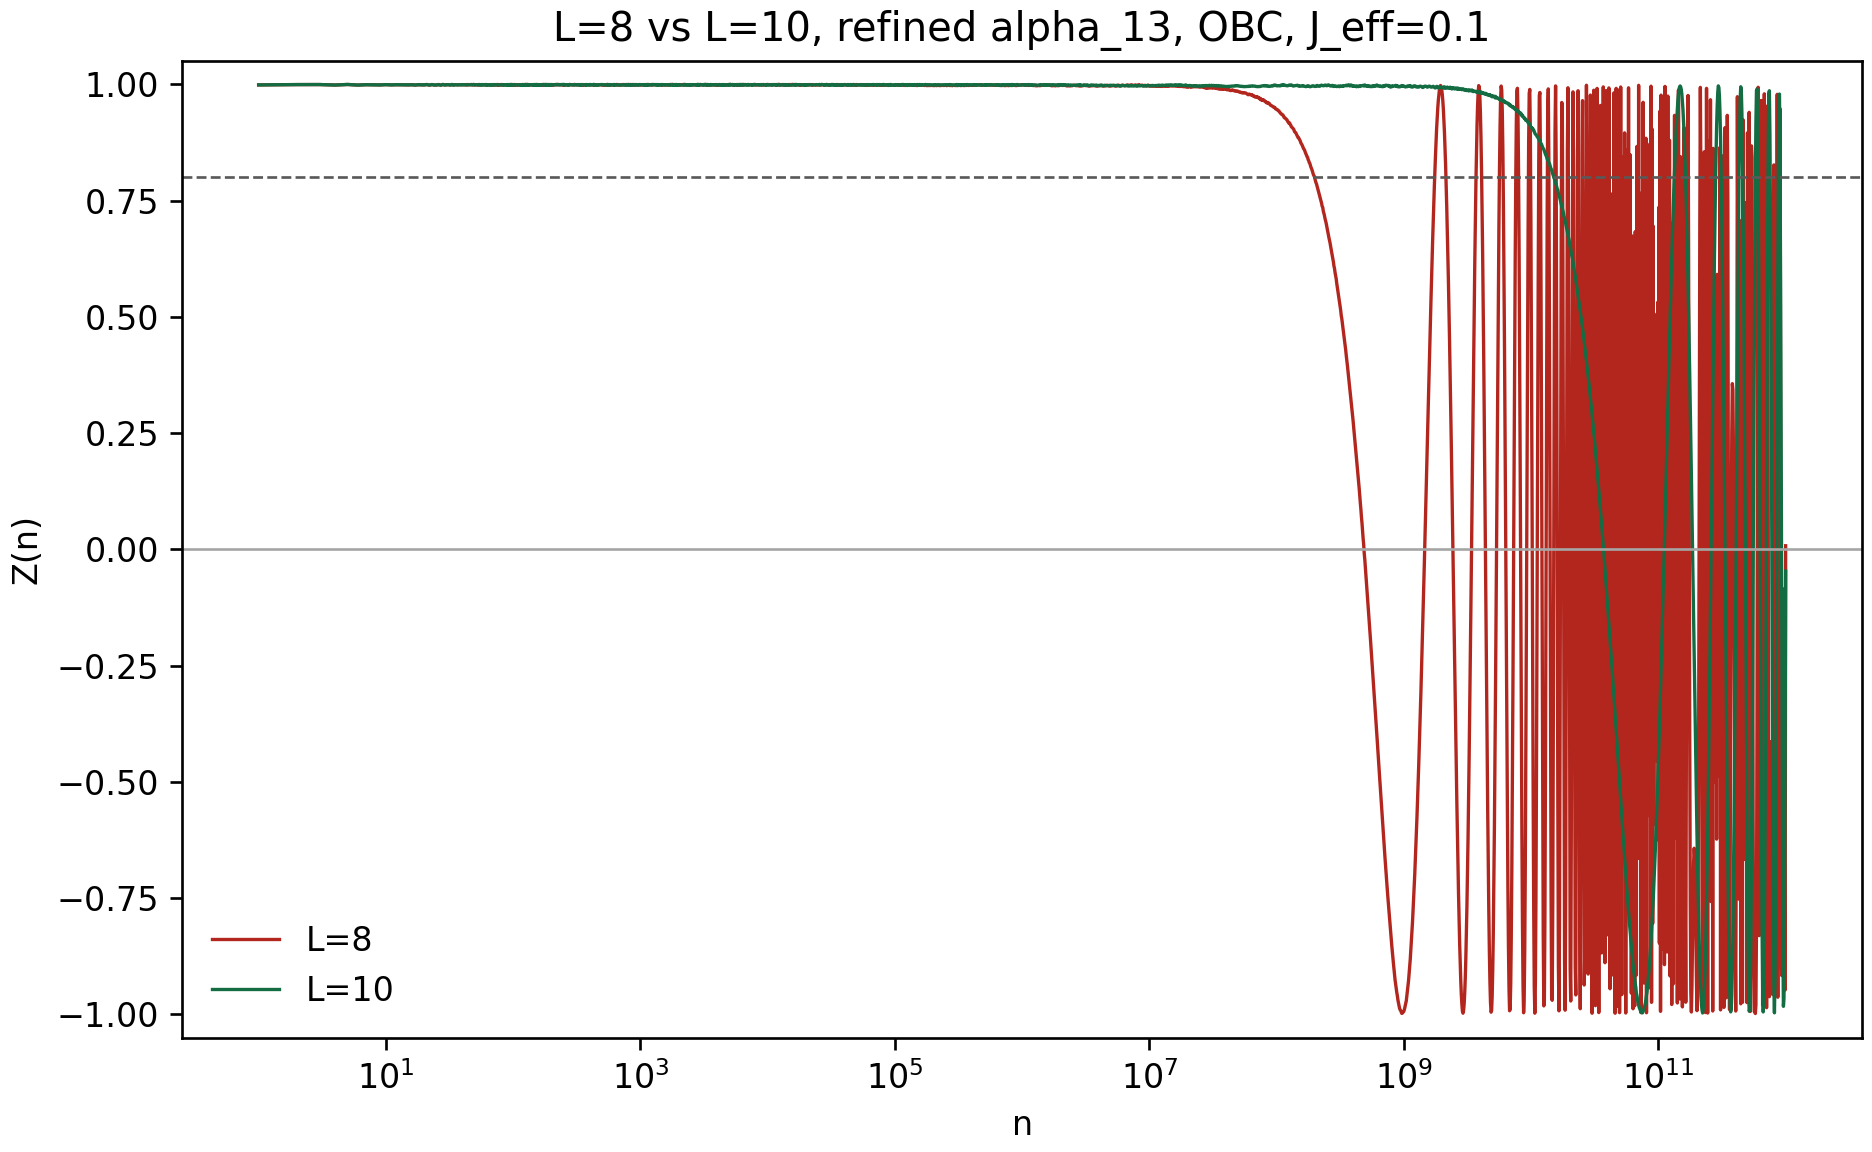
\includegraphics[width=0.98\linewidth]{l8_l10_alpha13_obc_comparison.png}
\caption{Current OBC size comparison for \(L=8\) and \(L=10\) at refined \(\alpha_{13}\), with \(J_{\rm eff}=0.1\). The \(L=10\) collapse is delayed by roughly two orders of magnitude relative to \(L=8\).}
\label{fig:size-alpha13}
\end{figure}

\subsection*{Possible Sources of the Detuned Discrepancy}

The size comparison separates two issues. The refined-\(\alpha_{13}\) result behaves as expected: increasing \(L\) delays the finite-size collapse. The detuned \(\alpha=81.60\) result does not. The most likely remaining explanations are:
\begin{itemize}
  \item \textbf{Interaction normalization is still not fully matched.} The \(J_{\rm eff}=0.1\) convention fixes the refined-\(\alpha_{13}\) early decay, but the detuned case may require the paper's exact spin-operator normalization or a different convention for the interaction energy scale.
  \item \textbf{The plotted raw \(Z(n)\) may not match the paper's lifetime extraction.} Fig.~4(c) discusses a drop to \(0.8\)--\(0.9\), a short plateau, and then a drastic fall. A raw sampled trace can cross thresholds early because of finite-size oscillations; an envelope, windowed average, or monotone decay estimator may be closer to the paper's procedure.
  \item \textbf{The initial-state or observable convention may differ subtly.} The current run uses the all-\(+x\) product state and the simple site average of \(\sigma_x\). A different product-state ensemble, disorder/phase averaging, or a slightly different normalization of \(m_x\) could suppress early oscillations.
  \item \textbf{Dense-Floquet exact finite-size spectra show revivals.} The method accurately resolves the finite Hilbert-space quasienergy spectrum. For small \(L\), this produces strong collapse and revival features, so a direct visual comparison to the paper may require matching the same smoothing and lifetime estimator.
\end{itemize}

\section{Generated Files}

The corrected run generated or updated:
\begin{itemize}
  \item \texttt{reproduce\_interacting.py};
  \item \texttt{params/interacting\_params\_local.json};
  \item \texttt{params/interacting\_params\_hpc.json};
  \item \texttt{params/interacting\_params\_periodic\_l10.json};
  \item \texttt{params/interacting\_params\_alpha81p60\_periodic\_l10.json};
  \item \texttt{params/interacting\_params\_alpha13\_obc\_n1e12\_l10.json};
  \item \texttt{data/diagnostics.json};
  \item \texttt{data/l10\_alpha13\_j\_convention\_check.json};
  \item \texttt{data/l10\_alpha13\_boundary\_check.json};
  \item \texttt{data/l10\_boundary\_and\_longtime\_checks.json};
  \item \texttt{data/l8\_l10\_size\_comparison\_current.json};
  \item \texttt{data/z\_stroboscopic\_alpha\_13\_l10.csv};
  \item \texttt{data/z\_stroboscopic\_alpha\_13\_l10\_n1e12.csv};
  \item \texttt{data/z\_stroboscopic\_alpha\_13\_l8\_n1e12\_current.csv};
  \item \texttt{data/z\_stroboscopic\_alpha\_81p60\_l10.csv};
  \item \texttt{data/z\_stroboscopic\_alpha\_81p60\_l8\_current.csv};
  \item \texttt{periodic\_l10/data/z\_stroboscopic\_alpha\_13\_l10\_periodic.csv};
  \item \texttt{periodic\_l10/data/z\_stroboscopic\_alpha\_81p60\_l10\_periodic.csv};
  \item \texttt{figures/l10\_alpha13\_j\_convention\_check.png};
  \item \texttt{figures/l10\_alpha13\_boundary\_check.png};
  \item \texttt{figures/l10\_alpha81p60\_boundary\_check.png};
  \item \texttt{figures/l10\_alpha13\_obc\_n1e12.png};
  \item \texttt{figures/l8\_l10\_alpha81p60\_obc\_comparison.png};
  \item \texttt{figures/l8\_l10\_alpha13\_obc\_comparison.png};
  \item \texttt{figures/z\_stroboscopic\_alpha\_13\_l10.png};
  \item \texttt{figures/z\_stroboscopic\_alpha\_81p60\_l10.png};
  \item compatibility copies without the \texttt{l10} suffix for older report references.
\end{itemize}

\section{How to Change Larger-System Parameters}

The main file to edit on the cluster is \texttt{params/interacting\_params\_hpc.json}. Keep the interaction convention lines:
\begin{verbatim}
"interaction_j": 0.2,
"interaction_operator_scale": 0.5,
\end{verbatim}
Then change the target length and period limits inside \texttt{stroboscopic}:
\begin{verbatim}
"stroboscopic": {
  "lengths": [12],
  "periods_by_alpha": {
    "alpha_81p60": 100000,
    "alpha_13": 10000000000
  },
  "steps_per_period": 120,
  "sampling_mode": "log_floquet",
  "floquet_integrator": "magnus4",
  "floquet_precision": "float64",
  "linear_prefix_periods": 200,
  "log_sample_count": 1600
}
\end{verbatim}
For \(L=12\), the dense Floquet matrix dimension is \(4096\), so the memory and matrix-exponential cost are much larger than for \(L=10\). A practical next run is \(L=12\) only after confirming the cluster memory headroom. If \(L=12\) becomes too slow, reduce only \texttt{steps\_per\_period} to \(60\) for a diagnostic run; the \(L=10\), \(\alpha_{13}\) result was stable across \(30\), \(60\), and \(120\) steps per period.

\section{Remaining Issue}

The refined \(\alpha_{13}\) early-decay problem is fixed. The detuned \(\alpha=81.60\) raw \(Z(n)\) points still decay too quickly compared with Fig.~4(c) if one reads the first raw threshold crossing directly. This is not yet a faithful reproduction of the detuned finite-size lifetime curve. The next scientific step is to check the remaining model conventions, especially boundary conditions and the interaction normalization, and then implement an explicit envelope or windowed lifetime estimator before comparing detuned finite-size scaling.

\end{document}
